% 第 3 章 Constraining Timing Paths
\bichapter{约束时序路径}{Constraining Timing Paths}\label{chap:paths}

时序路径是设计中的一条点到点序列：从寄存器时钟引脚或输入端口出发，经过组合逻辑，结束于寄存器数据输入引脚或输出端口。

下列主题说明时序路径，以及约束时序路径的相关任务：
\begin{itemize}
  \item 时序路径与 path group
  \item 创建 path group
  \item 同一 launch 与 capture 时钟的路径延迟分析
  \item 不同 launch 与 capture 时钟的路径延迟分析
  \item 输入延迟与输出延迟简介
  \item 为端口设置输入延迟与输出延迟
  \item 指定时序例外
  \item 指定 false path 例外
  \item 指定最大与最小路径延迟例外
  \item 指定 multicycle path 例外
  \item 指定路径时序裕量例外
  \item 高效地指定例外
  \item 例外的优先级
  \item 禁用下层 block 内部的时序路径
  \item 使用 case analysis
  \item 禁用时序弧
  \item 使能 preset 与 clear 时序
  \item data-to-data check 简介
  \item 指定 data-to-data check
  \item 使能基于库的 data check
  \item 时钟门控检查简介
  \item 指定时钟门控检查
\end{itemize}

\section{时序路径与 path group}
\subsection*{Timing Paths and Path Groups}

IC Compiler II 分析并优化设计中的时序路径。每条路径都有：
\begin{itemize}
  \item 起点（startpoint），数据在此被发射（launch）。\\
        路径起点是时序单元的时钟引脚，或设计的输入端口。有效时钟沿到达起点时，数据沿该路径被发射出去。输入端口也可以视为起点，因为数据由外部源发射后到达该端口。
  \item 终点（endpoint），数据穿过组合逻辑后在此被捕获（capture）。\\
        路径终点是时序单元的数据输入引脚，或设计的输出端口。有效时钟沿到达捕获器件的时钟输入时，路径末端的数据被捕获。输出端口也可以视为终点，因为离开该端口的数据由外部电路捕获。
\end{itemize}

下图给出一个设计及其时序路径的例子。

\begin{figure}[htbp]
  \centering
  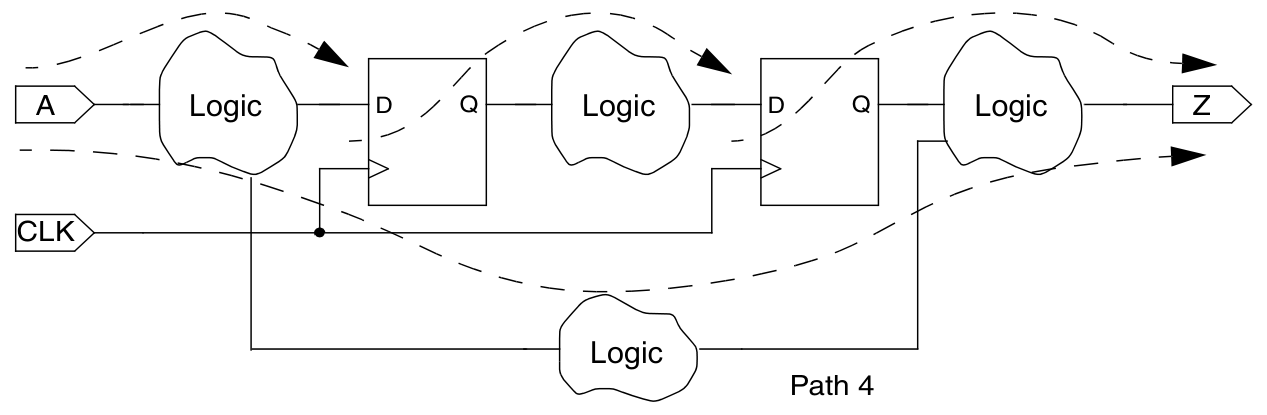
\includegraphics[width=0.9\textwidth]{fig-3-1.png}
  \caption{时序路径类型}
  \label{fig:3-1}
\end{figure}

每条路径都从数据发射点出发，经过若干组合逻辑，结束于数据捕获点：
\begin{itemize}
  \item 路径 1 从输入端口出发，结束于时序单元的数据输入。
  \item 路径 2 从时序单元的时钟引脚出发，结束于时序单元的数据输入。
  \item 路径 3 从时序单元的时钟引脚出发，结束于输出端口。
  \item 路径 4 从输入端口出发，结束于输出端口。
\end{itemize}

设计中的每条路径都有对应的时序裕量（slack）。slack 是时间值，可以为正、零或负。slack 最差的那一条路径称为关键路径（critical path）。它是负 slack 最大的路径；若没有时序违例，则是设计中全部路径里 slack 最小的那一条。

工具把时序路径组织成组，并按组分别做时序分析与优化。默认情况下，设计中的每个时钟对应一个 path group。终点由某个时钟打拍的全部时序路径，都属于该时钟的 path group。

工具还会创建一个名为 \cmd{**default**} 的 path group（名称中包含星号）。\cmd{**default**} 组收纳无法按终点所用时钟归类的路径，例如直通（feedthrough）路径与异步路径。

同一 path group 内的全部时序路径一起做时序优化，并从关键路径开始。

默认情况下，所有 path group 的权重相同；一组之内的路径与其他 path group 分开优化、分开报告。在每个 path group 内部，工具持续优化并改善关键路径的时序，直到组内另一条路径变得更加关键。

\section{创建 path group}
\subsection*{Creating Path Groups}

要改变 path group 中的路径，使用 \cmd{group\_path} 命令，方式如下：
\begin{itemize}
  \item 用 \opt{-name} 指定名称，创建新的 path group。
  \item 用 \opt{-name} 指定已有 path group 的名称，把路径加入该组。
  \item 用 \opt{-default} 把路径从当前 path group 移回它们所属的默认 path group。
\end{itemize}

用下列一种或多种方法标识时序路径：
\begin{itemize}
  \item 用 \opt{-from}、\opt{-rise\_from} 或 \opt{-fall\_from} 指定路径起点。
  \item 用 \opt{-through}、\opt{-rise\_through} 或 \opt{-fall\_through} 指定一个或多个经过点，这些选项可使用一次或多次。
  \item 用 \opt{-to}、\opt{-rise\_to} 或 \opt{-fall\_to} 指定路径终点。
\end{itemize}

可以用下列方式影响优化对 path group 的处理：
\begin{itemize}
  \item 用 \opt{-weight} 改变 path group 的权重。
  \item 用 \opt{-critical\_range} 指定关键范围，标出优化所针对的关键路径。
\end{itemize}

工具会处理 \opt{-critical\_range} 所指定范围内的全部关键路径，并从最关键的路径开始。

下面的例子创建一个名为 \cmd{slct} 的 path group，权重为 2.5，关键范围为 5，成员是从名为 \cmd{slct\_reg} 的寄存器出发的全部时序路径。随后把从名为 \cmd{slct\_nxt} 的输入端口出发的时序路径加入该 path group。接着，把从输入端口 \cmd{slct\_nxt} 出发、且同时经过引脚 \cmd{U29/A} 与 \cmd{U54/Y} 的路径从该组中移出，并送回它们的默认 path group。

\begin{lstlisting}
icc2_shell> group_path -name slct -weight 2.5 -critical_range 5 \
-from [get_cells slct_reg]
icc2_shell> group_path -name slct -from [get_ports slct_nxt]
icc2_shell> group_path -default [get_ports slct_nxt] \
 -through [get_pin U29/A]  -through [get_pin U54/Y]
\end{lstlisting}

用 \cmd{report\_path\_groups} 报告 path group 信息，用 \cmd{remove\_path\_groups} 删除 path group。

\section{同一 launch 与 capture 时钟的路径延迟分析}
\subsection*{Path Delay Analysis for the Same Launch and Capture Clock}

默认情况下，工具检查数据是否在 launch 事件之后的下一个 capture 时钟沿到达。对单时钟设计，launch 发生在一个时钟沿，capture 发生在下一个时钟沿。

下图说明，对于由同一时钟发射并捕获、且该时钟周期为 10 的路径，工具如何确定 setup 与 hold 约束。

\begin{figure}[htbp]
  \centering
  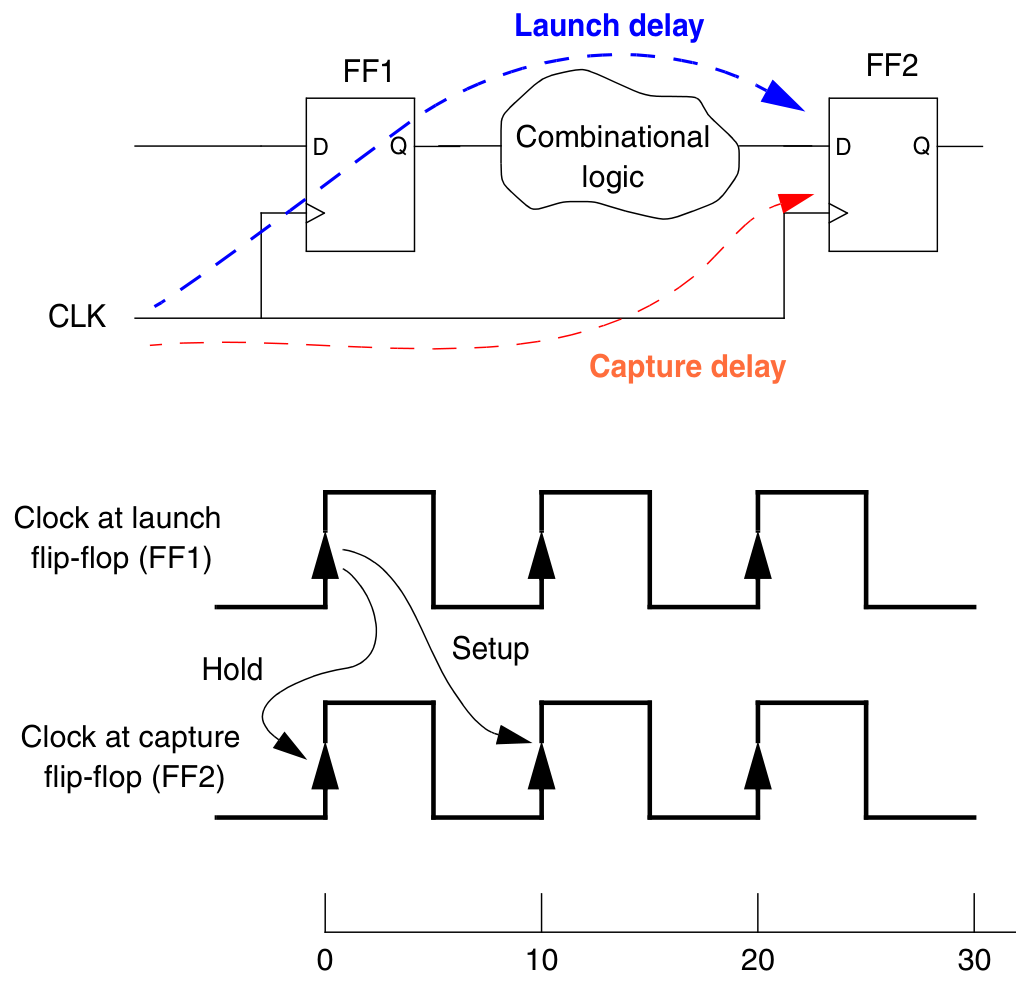
\includegraphics[width=0.9\textwidth]{fig-3-2.png}
  \caption{同一 launch 与 capture 时钟的 setup 与 hold 分析}
  \label{fig:3-2}
\end{figure}

时序分析期间，工具执行：
\begin{itemize}
  \item setup 检查，验证从 FF1 在时刻 0 发射的数据，能否及时到达 FF2 的 D 输入，以满足时刻 10 处 capture 沿的 setup 要求。\\
        若数据到达过晚、不能满足数据 setup 要求，工具报告 setup 违例。
  \item hold 检查，验证从 FF1 在时刻 0 发射的数据不会过早到达 FF2，即不会在 FF2 上一条数据满足 hold 要求之前到达。\\
        若数据到达过早，工具报告 hold 违例。
\end{itemize}

计算 launch 路径与 capture 路径上的延迟时，工具计入时钟网络效应带来的延迟，例如时钟源延迟（source latency）、网络延迟（network latency）以及时钟不确定性（clock uncertainty）。

\section{不同 launch 与 capture 时钟的路径延迟分析}
\subsection*{Path Delay Analysis for Different Launch and Capture Clocks}

对多时钟设计，工具默认假定所有时钟彼此同步，相位关系固定。时序分析时，若路径的 launch 时钟与 capture 时钟不同，工具考虑 launch 时钟沿之后最近的那个可能 capture 时钟沿，并据此确定该路径最紧的 setup 与 hold 要求。

下图给出一条由两个不同时钟分别发射和捕获的路径。

\begin{figure}[htbp]
  \centering
  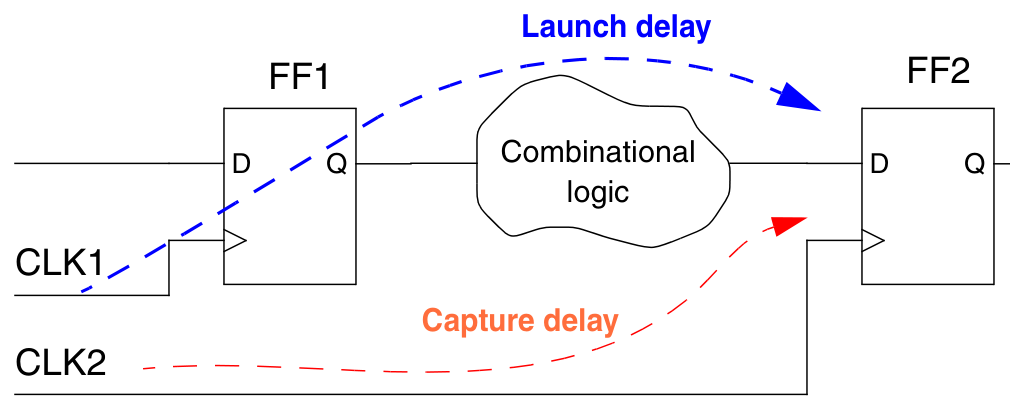
\includegraphics[width=0.9\textwidth]{fig-3-3.png}
  \caption{由不同时钟发射并捕获的路径}
  \label{fig:3-3}
\end{figure}

本例中的时钟 CLK1 与 CLK2 由下列命令创建：
\begin{lstlisting}
icc2_shell> create_clock -period 10 -waveform {0 5} CLK1
icc2_shell> create_clock -period 25 -waveform {5 12.5} CLK2
\end{lstlisting}

\subsection{不同 launch 与 capture 时钟的 setup 分析}
\subsubsection*{Setup Analysis for Different Launch and Capture Clocks}

launch 时钟与 capture 时钟不同时，工具在一段重复周期内考察两者有效沿之间的关系。这段时间长度是两个时钟周期的最小公倍数。对目标触发器的每一个 capture 沿，工具假定对应的 launch 沿是该 capture 沿之前最近的源时钟沿。

在下图中，工具考虑两种 launch 与 capture 沿的组合：
\begin{itemize}
  \item capture 沿在 time = 5，其之前最近的 launch 沿在 time = 0，标为 Setup 1。
  \item capture 沿在 time = 30，其之前最近的 launch 沿在 time = 20，标为 Setup 2。
\end{itemize}

\begin{figure}[htbp]
  \centering
  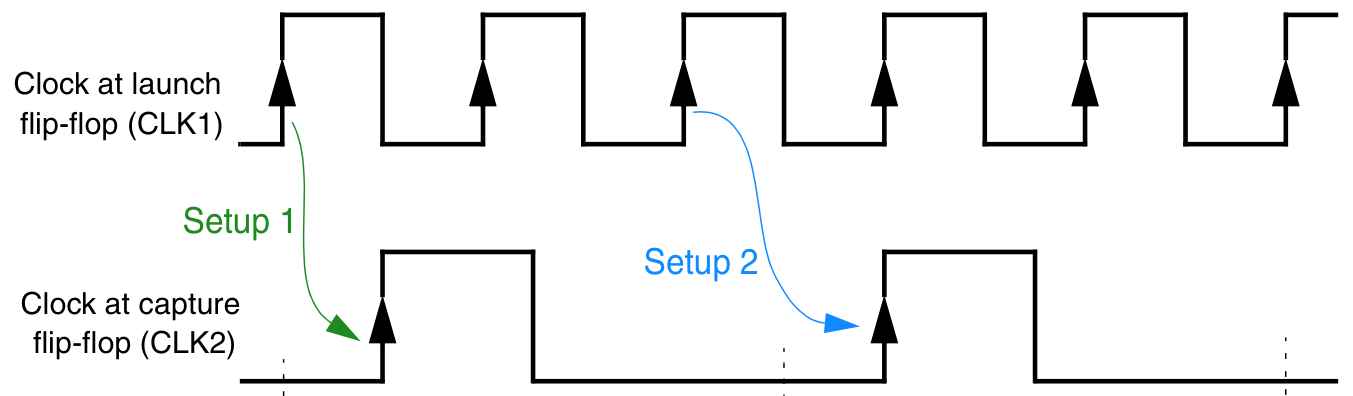
\includegraphics[width=0.9\textwidth]{fig-3-4.png}
  \caption{不同 launch 与 capture 时钟的 setup 分析}
  \label{fig:3-4}
\end{figure}

time = 30 的源时钟沿与 capture 沿同时发生，而不是更早，因此不把它当作对应的 launch 沿。

Setup 1 在 launch 与 capture 之间留出的时间更少，因此是更紧的约束，并决定该路径允许的最大延迟。本例中该值为 5。

\subsection{不同 launch 与 capture 时钟的 hold 分析}
\subsubsection*{Hold Analysis for Different Launch and Capture Clocks}

工具所检查的 hold 关系，基于用来确定 setup 关系的那些时钟沿的相邻沿。为确定最紧的 hold 关系，工具考虑全部有效的 setup 关系，包括下图中的 Setup 1 与 Setup 2。

\begin{figure}[htbp]
  \centering
  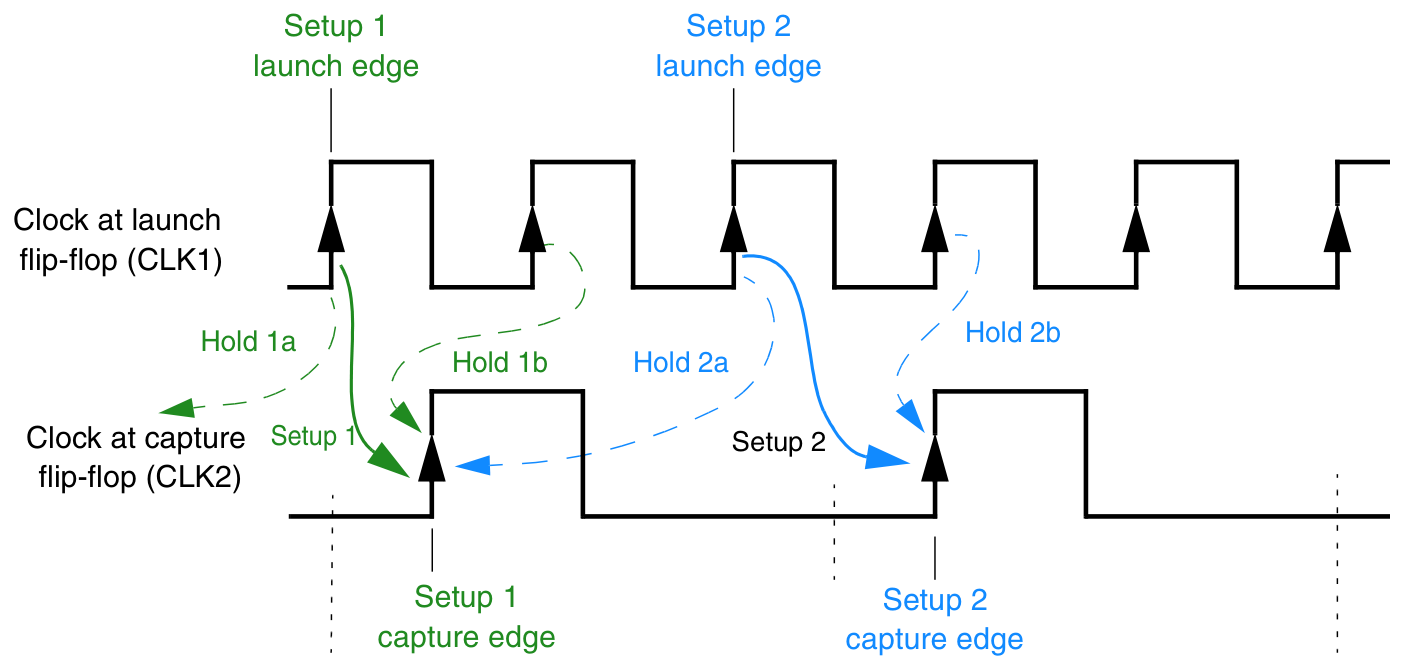
\includegraphics[width=0.9\textwidth]{fig-3-5.png}
  \caption{不同 launch 与 capture 时钟的 hold 分析}
  \label{fig:3-5}
\end{figure}

对每一种 setup 关系，工具做两种不同的 hold 检查：
\begin{itemize}
  \item 由该 setup 的 launch 沿发射的数据，不得被前一个 capture 沿捕获。
  \item 由下一个 launch 沿发射的数据，不得被该 setup 的 capture 沿捕获。
\end{itemize}

对标为 Setup 1 的 setup 关系，对应的两种 hold 检查标为 Hold1a 与 Hold1b。同样，对标为 Setup 2 的 setup 关系，两种 hold 检查标为 Hold2a 与 Hold2b。

在这些 hold 检查中，最紧的是 capture 沿相对 launch 沿发生得最晚的那一次，即 Hold 2b。因此 Hold 2b 决定该路径允许的最小延迟，本例中该值为 0。

\section{输入延迟与输出延迟简介}
\subsection*{Introduction to Input and Output Delays}

要分析一条时序路径，路径的起点和终点都必须受到约束。默认情况下，工具不知道数据到达输入端口的时刻，也不知道输出端口上数据的要求时刻。因此，要约束输入端口与输出端口，必须指定这些信息。

在下图中，到达名为 BlockA 的 block 的输入端口 A 的数据，由外部时序器件发射。

\begin{figure}[htbp]
  \centering
  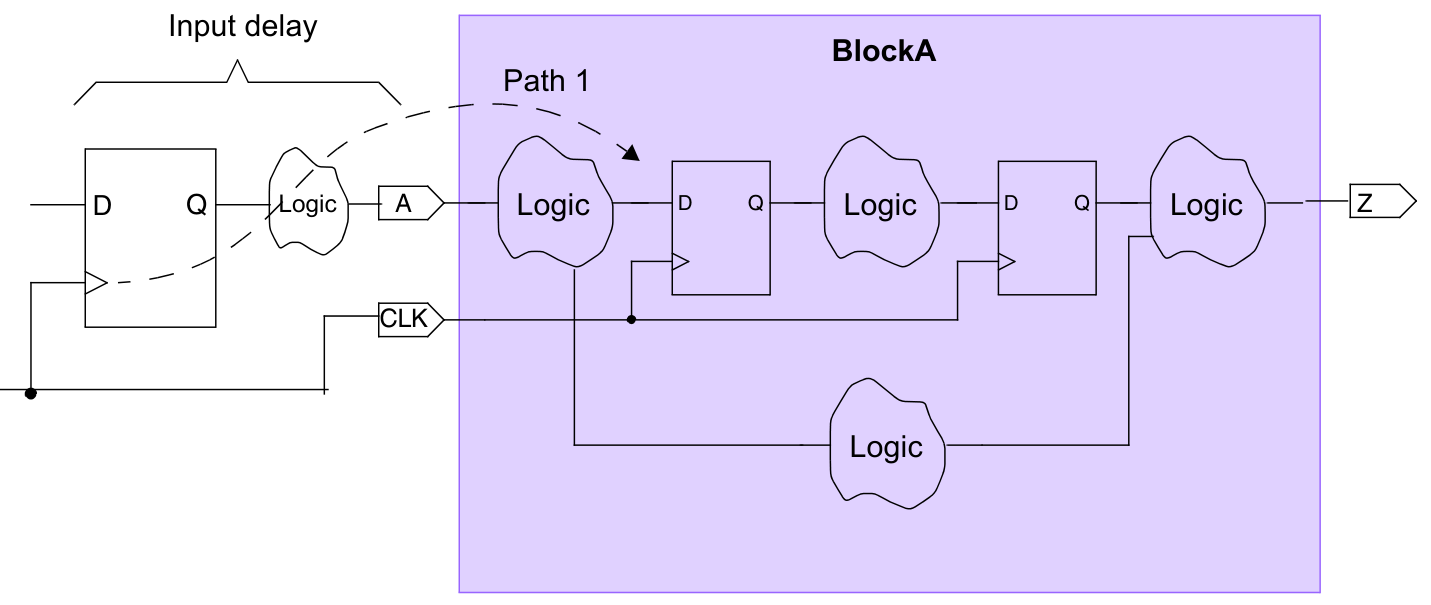
\includegraphics[width=0.9\textwidth]{fig-3-6.png}
  \caption{外部输入延迟}
  \label{fig:3-6}
\end{figure}

要约束输入端口 A，使用 \cmd{set\_input\_delay}，并指定：
\begin{itemize}
  \item 在外部时序器件上发射该数据的时钟。
  \item 数据被发射之后、到达该输入端口之前的延迟。
\end{itemize}

在下图中，离开名为 BlockA 的 block 的输出端口 Z 的数据，由外部时序器件捕获。

\begin{figure}[htbp]
  \centering
  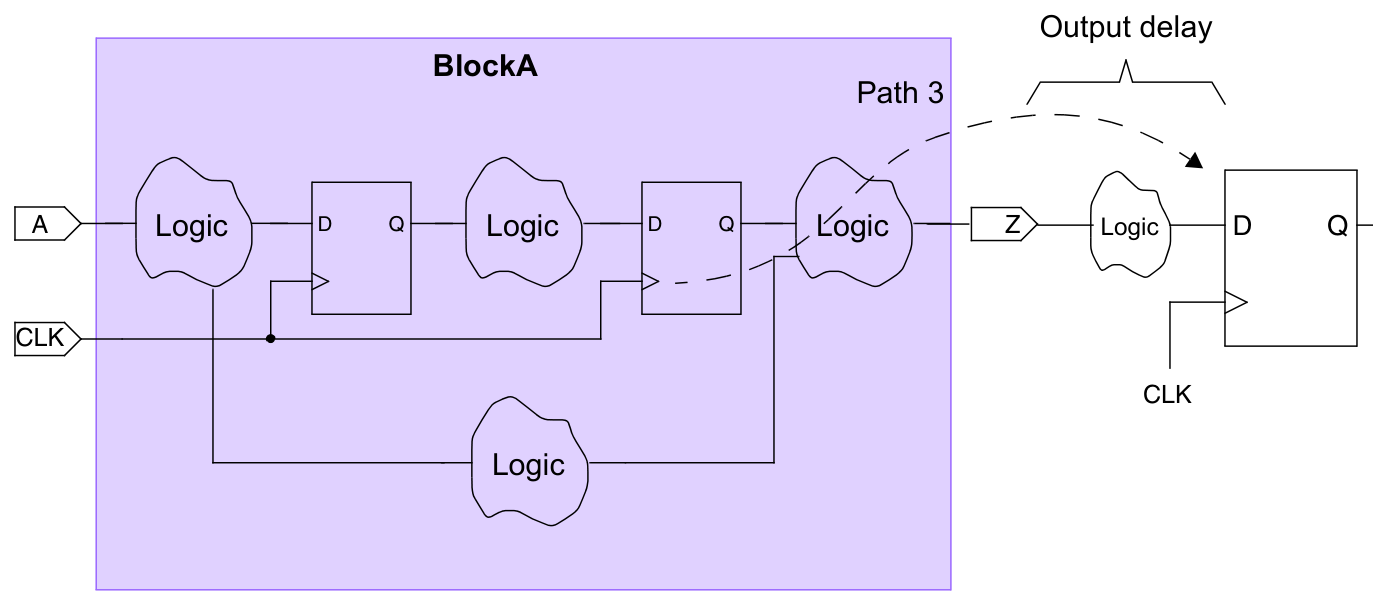
\includegraphics[width=0.9\textwidth]{fig-3-7.png}
  \caption{外部输出延迟}
  \label{fig:3-7}
\end{figure}

要约束输出端口 Z，使用 \cmd{set\_output\_delay}，并指定：
\begin{itemize}
  \item 在外部时序器件上捕获该数据的时钟。
  \item 数据离开端口 Z 之后、到达外部时序器件之前的延迟。
\end{itemize}

\section{为端口设置输入延迟与输出延迟}
\subsection*{Setting Input and Output Delays for Ports}

要靠指定端口外侧的外部延迟来约束输入或输出端口，使用 \cmd{set\_input\_delay} 或 \cmd{set\_output\_delay}。也可以用这两条命令在 block 内部的引脚上施加输入或输出延迟，从而使该引脚成为时序路径的起点或终点。

使用 \cmd{set\_input\_delay} 或 \cmd{set\_output\_delay} 时，必须指定下列信息：
\begin{itemize}
  \item 输入或输出延迟值。
  \item 所约束的端口或引脚。
\end{itemize}

为使时序分析更准确，用下列两种方法之一指定相关时钟：
\begin{itemize}
  \item 用 \opt{-clock} 给出参考时钟的名称。\\
        指定 \opt{-clock} 时，工具默认：
        \begin{itemize}
          \item 假定输入或输出延迟相对于该时钟的上升沿。若延迟相对于下降沿，把 \opt{-clock\_fall} 与 \opt{-clock} 一起使用。
          \item 把为参考时钟指定的 source latency 与 network latency，加到与该输入或输出延迟相关联的 launch 或 capture 路径上。\\
                若参考时钟的 source latency 与 network latency 已经包含在输入或输出延迟之中，使用 \opt{-source\_latency\_included} 与 \opt{-network\_latency\_included}。若参考时钟是 propagated clock，则忽略 \opt{-network\_latency\_included}。
        \end{itemize}
  \item 用 \opt{-reference\_pin} 指定参考时钟网络上的一个引脚或端口。\\
        指定 \opt{-reference\_pin} 时，工具默认：
        \begin{itemize}
          \item 用所有能够到达该参考引脚的时钟来约束端口。要选定某一个时钟，把 \opt{-clock} 与 \opt{-reference\_pin} 一起使用。
          \item 对到达该参考引脚的 ideal clock，把为该时钟指定的 source latency 与 network latency，加到与输入或输出延迟对应的 launch 或 capture 路径上。\\
                对到达该参考引脚的 propagated clock，工具把为该时钟指定的 source delay，以及传播到该参考引脚为止的时钟网络延迟，加到与输入或输出延迟对应的 launch 或 capture 路径上。
        \end{itemize}
\end{itemize}

若不指定相关时钟，工具根据当前 block 的时钟派生一个新时钟。

使用 \cmd{set\_input\_delay} 或 \cmd{set\_output\_delay} 时，可以指定该延迟：
\begin{itemize}
  \item 只用 \opt{-rise} 或 \opt{-fall} 作用于上升或下降跳变。\\
        默认情况下，工具把该延迟同时用于输入或输出端口上的上升与下降跳变。
  \item 只用 \opt{-max} 或 \opt{-min} 作用于最长或最短路径。\\
        默认情况下，工具把该延迟同时用于最长路径与最短路径。
  \item 用 \opt{-level\_sensitive} 相对于电平敏感锁存器。\\
        默认情况下，工具假定与该输入或输出延迟相关联的时序路径，由边沿敏感触发器发射或捕获。
  \item 用 \opt{-add\_delay} 不覆盖已有的输入或输出延迟设置。\\
        用该选项为同一端口相对于不同参考时钟指定不同的输入或输出延迟。
\end{itemize}

对具有多个 scenario 的设计，输入或输出延迟默认只作用于当前 scenario。要为其他范围指定输入或输出延迟：
\begin{itemize}
  \item 特定 mode 的全部 scenario：使用 \opt{-modes}。
  \item 特定 corner 的全部 scenario 以及当前 mode：使用 \opt{-corners}。
  \item 特定 mode 与 corner 的全部 scenario：同时使用 \opt{-modes} 与 \opt{-corners}。
  \item 特定 scenario：使用 \opt{-scenarios}。\\
        使用该选项时，不能同时使用 \opt{-modes} 或 \opt{-corners}。
\end{itemize}

要从端口上去掉输入或输出延迟，使用 \cmd{remove\_input\_delay} 或 \cmd{remove\_output\_delay}。

下图给出一个 block 的一个输入与一个输出的外部路径，以及与这些外部路径相关联的延迟。

\begin{figure}[htbp]
  \centering
  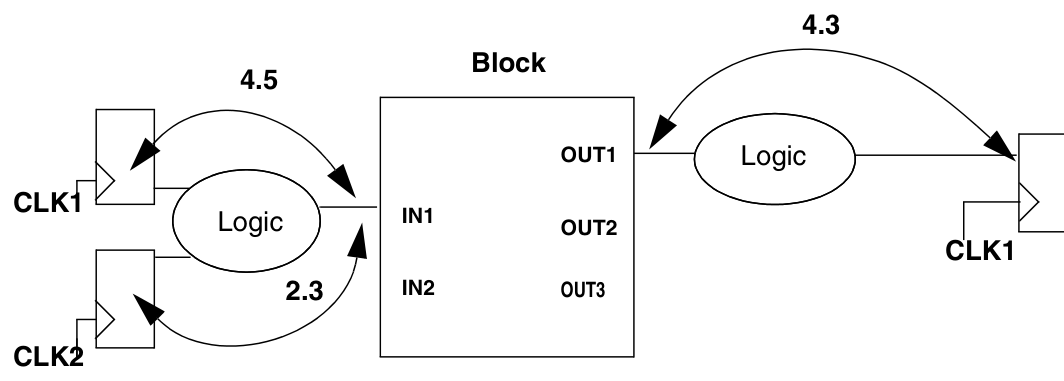
\includegraphics[width=0.9\textwidth]{fig-3-8.png}
  \caption{输入端口与输出端口的外部延迟}
  \label{fig:3-8}
\end{figure}

下列命令约束名为 IN1 的输入：相对于名为 CLK1 的时钟设置输入延迟 4.5，并相对于名为 CLK2 的时钟设置输入延迟 2.3。
\begin{lstlisting}
icc2_shell> set_input_delay 4.5 -clock CLK1 [get_ports IN1]
icc2_shell> set_input_delay 2.3 -clock CLK2 [get_ports IN1] \
 -add_delay
\end{lstlisting}

下列命令约束名为 OUT1 的输出：相对于名为 CLK1 的时钟设置输出延迟 4.3。
\begin{lstlisting}
icc2_shell> set_output_delay 4.3 -clock CLK1 [get_ports OUT1]
\end{lstlisting}

\subsection{考虑 driving cell 延迟的影响}
\subsubsection*{Considering the Effect of Delays Through Driving Cells}

若用 \cmd{set\_driving\_cell} 约束输入或 inout 端口，如下例所示，工具会把外部 driving cell 延迟中随负载变化的那一部分，计入从该端口开始的时序路径，如下图所示。
\begin{lstlisting}
icc2_shell> set_driving_cell -lib_cell AND2 -from_pin A [get_ports I1]
\end{lstlisting}

\begin{figure}[htbp]
  \centering
  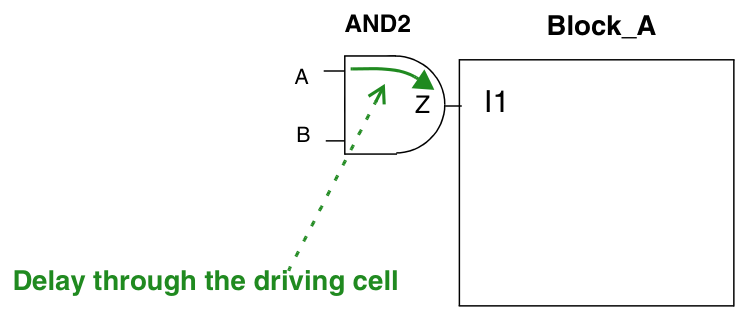
\includegraphics[width=0.9\textwidth]{fig-3-9.png}
  \caption{driving cell 上的延迟}
  \label{fig:3-9}
\end{figure}

为避免这段延迟被计算两次，先估计 driving cell 随负载变化的延迟，再从端口上指定的输入延迟中减去该值。

\subsection{时钟端口上 input delay 的影响}
\subsubsection*{Effect of Input Delay on Clock Ports}

若时钟是 propagated clock，工具把时钟源端口或引脚上的输入延迟当作 source latency。该输入延迟可以不相对于任何时钟，也可以相对于该源自身的时钟。source latency 值会加到时钟网络延迟上，得到总延迟（total latency）。

不要像下例这样对全部输入端口设置输入延迟：
\begin{lstlisting}
icc2_shell> set_input_delay 2 -clock CLK [all_inputs]
\end{lstlisting}

应当对除时钟端口以外的全部输入设置输入延迟，如下例所示：
\begin{lstlisting}
icc2_shell> set_input_delay 2 -clock CLK \
       [remove_from_collection [all_inputs] [get_ports CLK]]
\end{lstlisting}

若存在实际的 source latency，用带 \opt{-source} 的 \cmd{set\_clock\_latency} 来定义。

\section{指定时序例外}
\subsection*{Specifying Timing Exceptions}

IC Compiler II 允许设置下列类型的时序例外：
\begin{itemize}
  \item false path：标出不需要做时序分析的路径。\\
        使用 \cmd{set\_false\_path}，见“指定 false path 例外”。
  \item 最小与最大延迟值：在指定起点与终点之间设置最小与最大路径延迟要求。\\
        使用 \cmd{set\_max\_delay} 与 \cmd{set\_min\_delay}，见“指定最大与最小路径延迟例外”。
  \item multicycle path：用指定路径所需的时钟周期数，覆盖默认的单周期要求。\\
        使用 \cmd{set\_multicycle\_path}，见“指定 multicycle path 例外”。
  \item 路径时序裕量（path timing margin）：按指定的时间量收紧或放宽指定路径的时序要求。\\
        使用 \cmd{set\_path\_margin}，见“指定路径时序裕量例外”。
\end{itemize}

每条时序例外命令既可以作用于单条路径，也可以作用于一组相关路径，例如从一个时钟域到另一个时钟域的全部路径，或经过设计中某指定点的全部路径。

要报告已经施加到设计上的全部时序例外，使用 \cmd{report\_exceptions}。

要把路径恢复到施加时序例外之前的默认状态，使用 \cmd{reset\_paths}，或使用各时序例外命令的 \opt{-reset\_path} 选项。

\section{指定 false path 例外}
\subsection*{Specifying False Path Exceptions}

false path 是不需要做时序分析的路径。例如，两个经多路选择的逻辑块之间可以存在一条路径，但两者从不同时被选中，因此该路径对时序分析无效。把这类路径指定为 false path，可避免工具把时间花在分析真实设计中不会出现的时序路径上。

要用 \cmd{set\_false\_path} 把时序路径定义为 false path，必须用下列一种或多种方法指定要设置的路径：
\begin{itemize}
  \item 用 \opt{-from}、\opt{-rise\_from} 或 \opt{-fall\_from} 指定路径起点。\\
        有效起点为：
        \begin{itemize}
          \item 时钟。\\
                若指定时钟，则从该时钟所约束的全部时序单元与原始端口出发的时序路径都被设为 false path。
          \item 时序单元。
          \item 时序单元的时钟引脚。
          \item 锁存器的数据引脚。
          \item 输入或 inout 端口。
          \item 已设置 input delay 的引脚。
        \end{itemize}
  \item 用 \opt{-through}、\opt{-rise\_through} 或 \opt{-fall\_through} 指定一个或多个经过点，这些选项可使用一次或多次。\\
        有效经过点为：
        \begin{itemize}
          \item 引脚
          \item 端口
          \item 单元
          \item 线网
        \end{itemize}
        若经过某引脚的全部路径都是 false path，用 \cmd{set\_disable\_timing} 禁用该引脚的时序弧，比使用 \cmd{set\_false\_path} \opt{-through} 更高效。
  \item 用 \opt{-to}、\opt{-rise\_to} 或 \opt{-fall\_to} 指定路径终点。\\
        有效终点为：
        \begin{itemize}
          \item 时钟。\\
                若指定时钟，则结束于该时钟所约束的全部时序单元与原始端口的时序路径都被设为 false path。
          \item 时序单元。
          \item 时序单元的数据引脚。
          \item 输出或 inout 端口。
          \item 已设置 output delay 的引脚。
        \end{itemize}
\end{itemize}

可选地，可以把 false path 设置限制为：
\begin{itemize}
  \item 只用 \opt{-setup} 或 \opt{-hold} 作用于 setup 或 hold 分析。\\
        默认情况下，false path 设置同时作用于 setup 与 hold 分析。
  \item 只用 \opt{-rise} 或 \opt{-fall} 作用于上升或下降分析。\\
        默认情况下，false path 设置同时作用于上升与下降分析。
\end{itemize}

要去掉 false path 设置，使用 \cmd{set\_false\_path} \opt{-reset\_path} 或 \cmd{reset\_paths}。

下例把一条很具体的路径设为 false path：从寄存器时钟引脚出发，经过若干引脚，结束于寄存器数据引脚。
\begin{lstlisting}
icc2_shell> set_false_path -from [get_pins reg2/CP] \
  -through [get_pins U31/Z] -through [get_pins U15/Z] \
  -to [get_pins reg7/D]
\end{lstlisting}

下例把时钟 ck1 与 ck2 之间的全部时序路径设为 false path：
\begin{lstlisting}
icc2_shell> set_false_path -from [get_clocks ck1] \
          -to [get_clocks ck2]
icc2_shell> set_false_path -from [get_clocks ck2] \
          -to [get_clocks ck1]
\end{lstlisting}

对本例，另一种做法是用 \cmd{set\_clock\_groups} 把时钟 ck1 与 ck2 之间的全部路径排除在时序分析之外。

\section{指定最大与最小路径延迟例外}
\subsection*{Specifying Maximum and Minimum Path Delay Exceptions}

默认情况下，工具根据 launch 与 capture 时钟沿的时刻计算路径允许的最大与最小延迟。要用自己的具体延迟约束覆盖默认的最大或最小允许路径延迟，使用 \cmd{set\_max\_delay} 或 \cmd{set\_min\_delay}。也可以用这两条命令约束一条不受时钟约束的纯组合时序路径。

使用 \cmd{set\_max\_delay} 或 \cmd{set\_min\_delay} 时，必须指定：
\begin{itemize}
  \item 最大或最小延迟值。
  \item 要用下列一种或多种方法约束的路径：
        \begin{itemize}
          \item 用 \opt{-from}、\opt{-rise\_from} 或 \opt{-fall\_from} 指定路径起点。\\
                有效起点为：
                \begin{itemize}
                  \item 时钟。\\
                        若指定时钟，则从该时钟所约束的全部时序单元与原始端口出发的时序路径都施加该最大或最小延迟。
                  \item 时序单元。
                  \item 时序单元的时钟引脚。
                  \item 锁存器的数据引脚。
                  \item 输入或 inout 端口。
                  \item 已设置 input delay 的引脚。
                \end{itemize}
          \item 用 \opt{-through}、\opt{-rise\_through} 或 \opt{-fall\_through} 指定一个或多个经过点，这些选项可使用一次或多次。\\
                有效经过点为：
                \begin{itemize}
                  \item 引脚
                  \item 端口
                  \item 单元
                  \item 线网
                \end{itemize}
          \item 用 \opt{-to}、\opt{-rise\_to} 或 \opt{-fall\_to} 指定路径终点。\\
                有效终点为：
                \begin{itemize}
                  \item 时钟。\\
                        若指定时钟，则结束于该时钟所约束的全部时序单元与原始端口的时序路径都施加该最大或最小延迟。
                  \item 时序单元。
                  \item 时序单元的数据引脚。
                  \item 输出或 inout 端口。
                  \item 已设置 output delay 的引脚。
                \end{itemize}
        \end{itemize}
\end{itemize}

可选地，可以把最大或最小路径延迟设置限制为：
\begin{itemize}
  \item 只用 \opt{-setup} 或 \opt{-hold} 作用于 setup 或 hold 分析。\\
        默认情况下，它同时作用于 setup 与 hold 分析。
  \item 只用 \opt{-rise} 或 \opt{-fall} 作用于上升或下降分析。\\
        默认情况下，它同时作用于上升与下降分析。
\end{itemize}

若施加 \cmd{set\_max\_delay} 或 \cmd{set\_min\_delay} 的路径起点或终点受时钟约束，时序分析时工具会使用起点与终点的时钟延迟。要忽略起点与终点的时钟延迟，使用 \opt{-ignore\_clock\_latency}。

要去掉最大或最小路径延迟设置，使用 \cmd{set\_max\_delay} 或 \cmd{set\_min\_delay} 的 \opt{-reset\_path} 选项，或使用 \cmd{reset\_paths}。

下例把寄存器 REGA 与 REGB 之间的最大路径延迟设为 12，最小路径延迟设为 2：
\begin{lstlisting}
icc2_shell> set_max_delay 12.0 \
          -from [get_cells REGA] -to [get_cells REGB]
icc2_shell> set_min_delay 2.0 \
          -from [get_cells REGA] -to [get_cells REGB]
\end{lstlisting}

\section{指定 multicycle path 例外}
\subsection*{Specifying Multicycle Path Exceptions}

若数据从路径起点传播到终点所需的时钟周期数，多于工具使用的单周期要求，可以用 \cmd{set\_multicycle\_path} 为该路径指定额外的时钟周期。随后工具按指定的周期数计算 setup 或 hold 约束。

使用 \cmd{set\_multicycle\_path} 时，必须指定：
\begin{itemize}
  \item 要为该路径分配的时钟周期数。\\
        若路径的 launch 时钟与 capture 时钟不是同一个时钟，用 \opt{-start} 或 \opt{-end} 说明周期数基于 launch 时钟还是 capture 时钟。默认情况下，工具相对于 capture 时钟移动 setup 检查，相对于 launch 时钟移动 hold 检查。
  \item 要用下列一种或多种方法约束的路径：
        \begin{itemize}
          \item 用 \opt{-from}、\opt{-rise\_from} 或 \opt{-fall\_from} 指定路径起点。\\
                有效起点为：
                \begin{itemize}
                  \item 时钟。\\
                        若指定时钟，则从该时钟所约束的全部时序单元与原始端口出发的时序路径都施加该多周期设置。
                  \item 时序单元。
                  \item 时序单元的时钟引脚。
                  \item 锁存器的数据引脚。
                  \item 输入或 inout 端口。
                  \item 已设置 input delay 的引脚。
                \end{itemize}
          \item 用 \opt{-through}、\opt{-rise\_through} 或 \opt{-fall\_through} 指定一个或多个经过点，这些选项可使用一次或多次。\\
                有效经过点为：
                \begin{itemize}
                  \item 引脚
                  \item 端口
                  \item 单元
                  \item 线网
                \end{itemize}
          \item 用 \opt{-to}、\opt{-rise\_to} 或 \opt{-fall\_to} 指定路径终点。\\
                有效终点为：
                \begin{itemize}
                  \item 时钟。\\
                        若指定时钟，则结束于该时钟所约束的全部时序单元与原始端口的时序路径都施加该多周期设置。
                  \item 时序单元。
                  \item 时序单元的数据引脚。
                  \item 输出或 inout 端口。
                  \item 已设置 output delay 的引脚。
                \end{itemize}
        \end{itemize}
\end{itemize}

可选地，可以把 multicycle path 设置限制为：
\begin{itemize}
  \item 只用 \opt{-setup} 或 \opt{-hold} 作用于 setup 或 hold 分析。\\
        默认情况下，它同时作用于 setup 与 hold 分析。\\
        工具对 \cmd{set\_multicycle\_path} 中 \opt{-setup} 与 \opt{-hold} 的数值解释不同。\opt{-setup} 参数的整数值指定 multicycle path 的时钟周期数。没有时序例外时，默认值为 1。\opt{-hold} 参数的整数值指定：相对于有效 setup 关系，把 capture 沿从默认位置向后移动的时钟周期数。默认值为 0。
  \item 只用 \opt{-rise} 或 \opt{-fall} 作用于上升或下降分析。\\
        默认情况下，它同时作用于上升与下降分析。
\end{itemize}

要去掉 multicycle path 设置，使用 \cmd{set\_multicycle\_path} \opt{-reset\_path} 或 \cmd{reset\_paths}。

\subsection{为 hold 分析指定正确的周期数}
\subsubsection*{Specifying the Correct Number of Multicycles for Hold Analysis}

下面的例子说明：当已经知道 setup 分析所需的周期数时，如何确定 hold 分析所需的正确周期数。

本例中，名为 Reg4 与 Reg5 的寄存器之间的时序路径按两个时钟周期设计。默认情况下，工具对所有路径都按单周期时序处理。因此需要用下列命令为这条路径指定时序例外。

要为该 block 设置 multicycle path，使用下列命令：
\begin{lstlisting}
icc2_shell> set_multicycle_path -setup 2 \
          -from [get_cells Reg4] -to [get_cells Reg5]
\end{lstlisting}

该命令指定这条路径占用两个时钟周期，并建立下图所示的新 setup 关系。launch 沿之后的第二个 capture 沿，成为路径终点所适用的沿。

\begin{figure}[htbp]
  \centering
  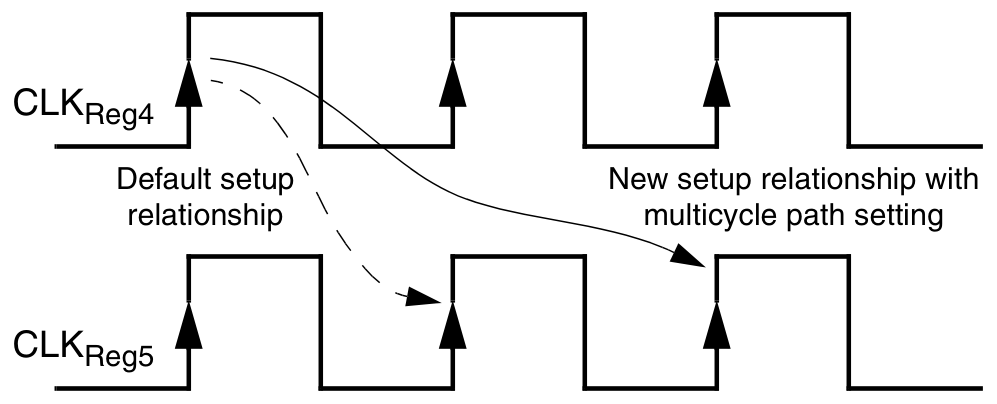
\includegraphics[width=0.9\textwidth]{fig-3-10.png}
  \caption{多周期路径的 setup}
  \label{fig:3-10}
\end{figure}

改变 setup 关系也会隐含地改变 hold 关系，因为所有 hold 关系都基于有效的 setup 关系。工具验证：由 setup 的 launch 沿发射的数据，不会被前一个 capture 沿捕获。新的 hold 关系如下图所示。

\begin{figure}[htbp]
  \centering
  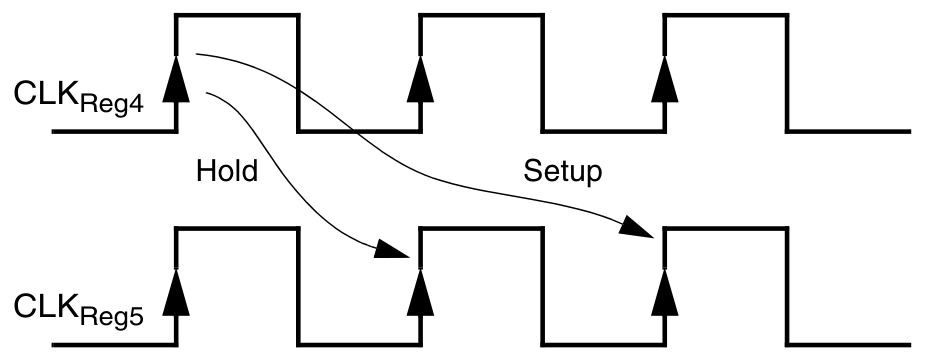
\includegraphics[width=0.9\textwidth]{fig-3-11.png}
  \caption{基于新 setup 关系的多周期路径 hold}
  \label{fig:3-11}
\end{figure}

图中所示的 hold 关系多半不是该设计的正确关系。若 Reg4 不需要把数据保持到第一个时钟沿之后，就必须指定 multicycle hold 时序例外，命令如下：
\begin{lstlisting}
icc2_shell> set_multicycle_path -setup 2 \
          -from [get_cells Reg4] -to [get_cells Reg5]
icc2_shell> set_multicycle_path -hold 1 \
          -from [get_cells Reg4] -to [get_cells Reg5]
\end{lstlisting}

下图给出用这两条 \cmd{set\_multicycle\_path} 正确设置后的 setup 与 hold 关系。第二条 \cmd{set\_multicycle\_path} 把 hold 关系的 capture 沿向后移动一个时钟周期，从虚线箭头移到实线箭头。

\begin{figure}[htbp]
  \centering
  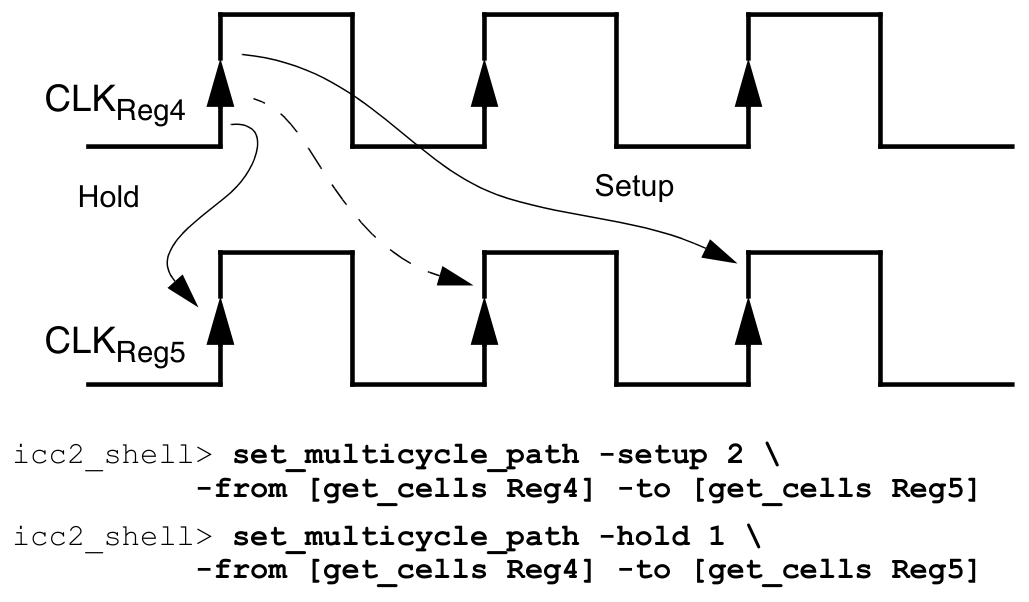
\includegraphics[width=0.9\textwidth]{fig-3-12.png}
  \caption{正确设置的多周期路径 hold}
  \label{fig:3-12}
\end{figure}

工具按下列公式确定 hold 周期数：

\begin{center}
\texttt{(hold cycles) = (setup option value) - 1 - (hold option value)}
\end{center}

默认情况下，hold cycles = 1 - 1 - 0 = 0。本例中 hold cycles = 2 - 1 - 1 = 0，这给出默认的 hold 行为。

\section{指定路径时序裕量例外}
\subsection*{Specifying Path Timing Margin Exceptions}

可以用 \cmd{set\_path\_margin} 使指定路径的时序检查按给定的时间量变得更松或更紧。

使用 \cmd{set\_path\_margin} 时，必须指定：
\begin{itemize}
  \item 裕量值。\\
        正值使检查更紧（more restrictive）。负值使检查更松（less restrictive）。
  \item 要用下列一种或多种方法约束的路径：
        \begin{itemize}
          \item 用 \opt{-from}、\opt{-rise\_from} 或 \opt{-fall\_from} 指定路径起点。\\
                有效起点为：
                \begin{itemize}
                  \item 时钟。\\
                        若指定时钟，则从该时钟所约束的全部时序单元与原始端口出发的时序路径都施加该路径裕量。
                  \item 时序单元。
                  \item 时序单元的时钟引脚。
                  \item 锁存器的数据引脚。
                  \item 输入或 inout 端口。
                  \item 已设置 input delay 的引脚。
                \end{itemize}
          \item 用 \opt{-through}、\opt{-rise\_through} 或 \opt{-fall\_through} 指定一个或多个经过点，这些选项可使用一次或多次。\\
                有效经过点为：
                \begin{itemize}
                  \item 引脚
                  \item 端口
                  \item 单元
                  \item 线网
                \end{itemize}
          \item 用 \opt{-to}、\opt{-rise\_to} 或 \opt{-fall\_to} 指定路径终点。\\
                有效终点为：
                \begin{itemize}
                  \item 时钟。\\
                        若指定时钟，则结束于该时钟所约束的全部时序单元与原始端口的时序路径都施加该路径裕量。
                  \item 时序单元。
                  \item 时序单元的数据引脚。
                  \item 输出或 inout 端口。
                  \item 已设置 output delay 的引脚。
                \end{itemize}
        \end{itemize}
\end{itemize}

可选地，可以把路径裕量设置限制为：
\begin{itemize}
  \item 只用 \opt{-setup} 或 \opt{-hold} 作用于 setup 或 hold 分析。\\
        默认情况下，它同时作用于 setup 与 hold 分析。
  \item 只用 \opt{-rise} 或 \opt{-fall} 作用于上升或下降分析。\\
        默认情况下，它同时作用于上升与下降分析。
\end{itemize}

要去掉路径裕量设置，使用 \cmd{set\_path\_margin} \opt{-reset\_path}。

下例使从单元 Reg4 到单元 Reg5 的全部 setup 检查收紧 1.2 个时间单位。
\begin{lstlisting}
icc2_shell> set_path_margin 1.2 \
   -from [get_cells Reg4] -to [get_cells Reg5]
\end{lstlisting}

所指定的裕量是在同一路径上已有的 minimum-delay、maximum-delay 与 multicycle path 例外之外，再叠加到时序检查上。施加在同一路径上的 false path 例外优先于路径时序裕量例外，裕量设置因此被忽略。

\section{高效地指定例外}
\subsection*{Specifying Exceptions Efficiently}

很多情况下，例外路径可以用许多不同方式指定。为缩短时序分析的运行时间，指定例外时遵循下列准则：
\begin{itemize}
  \item 先看清使例外成为必要的根本原因，再为受影响的路径找到控制时序分析的最简单方法。
  \item 在使用 false path 之前，考虑：
        \begin{itemize}
          \item 用 \cmd{set\_case\_analysis} 设置 case analysis。
          \item 用 \cmd{set\_clock\_groups} 声明时钟之间的互斥关系。
          \item 用 \cmd{set\_disable\_timing} 禁用设计中某一部分的分析。
        \end{itemize}
        这些替代方法可以比 \cmd{set\_false\_path} 更高效。
  \item 若必须设置 false path，避免用 \opt{-through} 或通配符指定大量路径。
\end{itemize}

例如，考虑下图所示电路。三个 16 位寄存器分别由三个不同时钟打拍。每个寄存器代表 16 个触发器。寄存器 REG2 只用于测试，因此电路正常工作时，从 REG2 到 REG3 的全部路径都是 false path。

\begin{figure}[htbp]
  \centering
  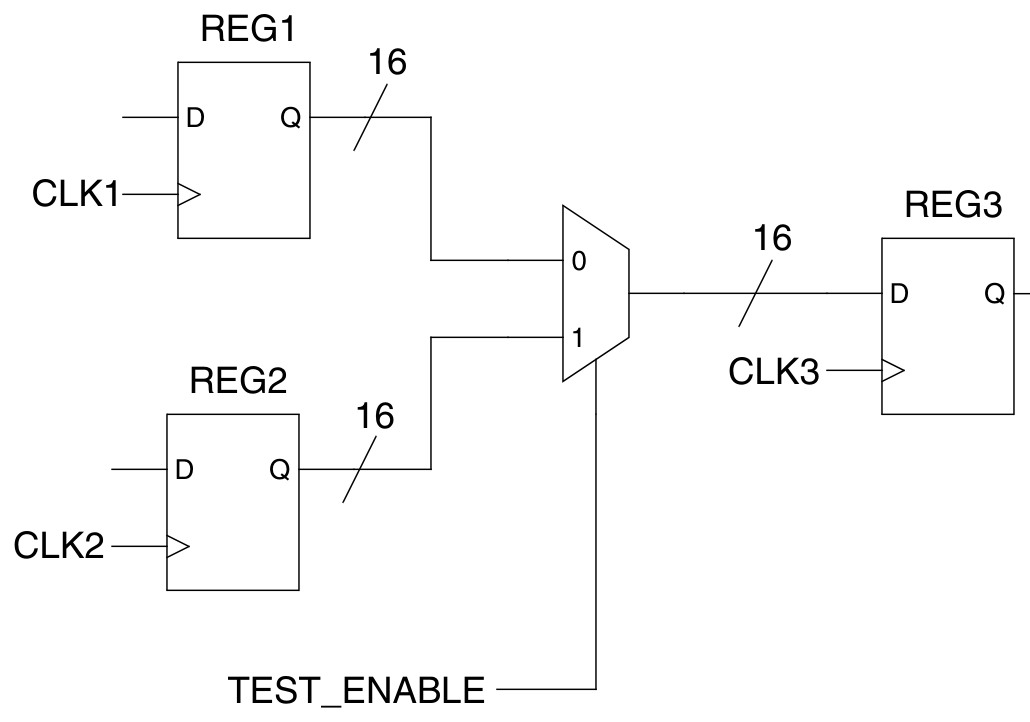
\includegraphics[width=0.9\textwidth]{fig-3-13.png}
  \caption{经过多路选择的寄存器路径}
  \label{fig:3-13}
\end{figure}

要忽略从 REG2 到 REG3 的时序，可以使用下列任一方法：
\begin{itemize}
  \item 用 case analysis 考虑测试使能信号为 0 的情形。
  \item 在 CLK1 与 CLK2 时钟域之间设置互斥关系。
  \item 把时钟域 CLK2 与 CLK3 之间的路径声明为 false。
\begin{lstlisting}
icc2_shell> set_false_path \
          -from [get_clocks CLK2] -to [get_clocks CLK3]
\end{lstlisting}
        这种方法指定 false path 的效率较高，因为工具只需要记录所指定的时钟域，不必记录寄存器、引脚、线网等对象上的例外。
  \item 把从 REG2 到 REG3 的 16 条单独路径声明为 false。
\begin{lstlisting}
icc2_shell> set_false_path -from [get_pins REG2[0]/CP] \
          -to [get_pins REG3[0]/D]
icc2_shell> set_false_path -from [get_pins REG2[1]/CP] \
          -to [get_pins REG3[1]/D]
icc2_shell> ...
\end{lstlisting}
        这种方法效率较低，因为工具必须记录 16 条不同路径上的时序例外。
  \item 把从 REG2 到 REG3 的全部路径声明为 false。
\begin{lstlisting}
icc2_shell> set_false_path -from [get_pins REG2[*]/CP] \
          -to [get_pins REG3[*]/D]
\end{lstlisting}
        这种方法效率更低，因为工具必须记录从 REG2 的每个时钟引脚到 REG3 的每个数据引脚的路径，共 256 条。
  \item 把从 REG2 出发的全部路径声明为 false。
\begin{lstlisting}
icc2_shell> set_false_path -from [get_pins REG2[*]/CP]
\end{lstlisting}
        这种方法与前一种类似。工具必须记录从 REG2 每个时钟引脚出发的全部路径，共 256 条。
\end{itemize}

\section{例外的优先级}
\subsection*{Order of Precedence for Exceptions}

对给定 block 中的每一条时序路径，工具找出适用于该路径的全部时序例外。若某条路径适用多个时序例外，实际用于该路径的例外取决于：
\begin{itemize}
  \item 所指定的例外类型，见“按例外类型的优先级”。
  \item 设置例外时使用的路径指定方法，见“按路径指定方式的优先级”。
\end{itemize}

\subsection{按例外类型的优先级}
\subsubsection*{Precedence Based on Exception Type}

下列几对时序例外类型不视为冲突，因此两种设置对一条路径都可以有效：
\begin{itemize}
  \item 两个 \cmd{set\_false\_path} 设置。
  \item \cmd{set\_min\_delay} 与 \cmd{set\_max\_delay} 设置。
  \item \cmd{set\_multicycle\_path} 的 \opt{-setup} 与 \opt{-hold} 设置。
  \item \cmd{set\_path\_margin} 与 \cmd{set\_min\_delay}、\cmd{set\_max\_delay} 或 \cmd{set\_multicycle\_path} 设置。
\end{itemize}

发生冲突时，时序例外类型按下列优先级从高到低排列：
\begin{enumerate}
  \item \cmd{set\_false\_path} 设置
  \item \cmd{set\_max\_delay} 与 \cmd{set\_min\_delay} 设置
  \item \cmd{set\_multicycle\_path} 设置
\end{enumerate}

例如，若把一条路径声明为 false，同时又把它的最大延迟设为某个值，则 false path 声明优先，最大延迟设置被忽略。

\subsection{按路径指定方式的优先级}
\subsubsection*{Precedence Based on Path Specification}

施加在更具体对象（例如引脚或端口）上的时序例外，优先于施加在更一般对象（例如时钟）上的同类例外。

各种路径指定方法按下列优先级从高到低排列：
\begin{enumerate}
  \item \opt{-from} pin、\opt{-rise\_from} pin、\opt{-fall\_from} pin 设置
  \item \opt{-to} pin、\opt{-rise\_to} pin、\opt{-fall\_to} pin 设置
  \item \opt{-through}、\opt{-rise\_through}、\opt{-fall\_through} 设置
  \item \opt{-from} clock、\opt{-rise\_from} clock、\opt{-fall\_from} clock 设置
  \item \opt{-to} clock、\opt{-rise\_to} clock、\opt{-fall\_to} clock 设置
\end{enumerate}

按上述优先级规则，若干可能的路径指定组合从高到低如下：
\begin{enumerate}
  \item \opt{-from} pin \opt{-to} pin
  \item \opt{-from} pin \opt{-to} clock
  \item \opt{-from} pin
  \item \opt{-from} clock \opt{-to} pin
  \item \opt{-to} pin
  \item \opt{-from} clock \opt{-to} clock
  \item \opt{-from} clock
  \item \opt{-to} clock
\end{enumerate}

例如，假定设置了下列例外：
\begin{lstlisting}
icc2_shell> set_max_delay 12 -from [get_clocks CLK1]
icc2_shell> set_max_delay 15 -from [get_clocks CLK1] -to [get_clocks CLK2]
\end{lstlisting}

第一条命令设置从 CLK1 出发的全部路径的最大延迟。第二条命令更具体，因此对从 CLK1 出发并结束于 CLK2 的路径，它覆盖第一条命令。

\subsection{例外优先级示例}
\subsubsection*{Example on the Order of Precedence of Exceptions}

假定一个具有四个时钟 clkA、clkB、clkC 与 clkD 的 block 上有下列例外设置：
\begin{lstlisting}
icc2_shell> set_false_path \
          -from [get_clocks clkB] -to [get_clocks clkC]
icc2_shell> set_multicycle_path  2 \
          -from [get_clocks clkA] -to [get_clocks clkC]
icc2_shell> set_multicycle_path 3 -to [get_pins Reg53/D]
icc2_shell> set_multicycle_path 3 -from [get_pins Reg24/CK]
\end{lstlisting}

对一条从单元 Reg24 出发、结束于单元 Reg32 的时序路径，Reg24 由时钟 clkB 打拍，Reg32 由时钟 clkD 打拍，只有下列例外适用：
\begin{lstlisting}
icc2_shell> set_multicycle_path 3 -from [get_pins Reg24/CK]
\end{lstlisting}

对一条从单元 Reg24 出发、结束于单元 Reg11 的时序路径，Reg24 由时钟 clkB 打拍，Reg11 由时钟 clkC 打拍，下列两个例外都适用：
\begin{lstlisting}
icc2_shell> set_false_path \
          -from [get_clocks clkB] -to [get_clocks clkC]
icc2_shell> set_multicycle_path 3 -from [get_pins Reg24/CK]
\end{lstlisting}

此时 \cmd{set\_false\_path} 优先于 \cmd{set\_multicycle\_path}，因此工具对该路径使用 false path 例外。

对一条从单元 Reg61 出发、结束于单元 Reg53 的时序路径，Reg61 由时钟 clkA 打拍，Reg53 由时钟 clkC 打拍，下列两个例外都适用：
\begin{lstlisting}
icc2_shell> set_multicycle_path  2 \
          -from [get_clocks clkA] -to [get_clocks clkC]
icc2_shell> set_multicycle_path 3 -to [get_pins Reg53/D]
\end{lstlisting}

此时有两条路径指定方式不同的 \cmd{set\_multicycle\_path}，工具采用更具体的路径指定，即到单元 Reg53 的 D 引脚的 multicycle path 设置。

\section{禁用下层 block 内部的时序路径}
\subsection*{Disabling Timing Paths Within Lower-Level Blocks}

对带层次的设计，可以用 \cmd{set\_timing\_paths\_disabled\_blocks} 禁用完全位于下层 block 内部的时序路径，使其不参与时序分析与优化。

要禁用完全位于下列范围之内的时序路径：
\begin{itemize}
  \item 指定的子 block：使用 \opt{-blocks}。
  \item 全部子 block：使用 \opt{-all\_sub\_blocks}。
\end{itemize}

要恢复子 block 内被禁用的时序路径，使用 \cmd{remove\_timing\_paths\_disabled\_blocks}。

\section{使用 case analysis}
\subsection*{Using Case Analysis}

case analysis 让你在端口或引脚上使用逻辑常量或逻辑跳变做时序分析，从而限制在设计中传播的信号。

若 case analysis 设置为：
\begin{itemize}
  \item 逻辑常量，工具禁用该常量所传播到的路径。\\
        使用 \cmd{set\_case\_analysis 0} 或 \cmd{set\_case\_analysis 1}，如下例所示：
\begin{lstlisting}
icc2_shell> set_case_analysis 0 [get_ports TEST_EN]
\end{lstlisting}
  \item 逻辑跳变，上升或下降，工具通过限制分析时所考虑的跳变来消除某些路径。\\
        使用 \cmd{set\_case\_analysis rising} 或 \cmd{set\_case\_analysis falling}，如下例所示：
\begin{lstlisting}
icc2_shell> set_case_analysis rising [get_ports RESET]
\end{lstlisting}
\end{itemize}

此外，工具还把下列情形也当作 case analysis 值：
\begin{itemize}
  \item 连接到 tie-high 或 tie-low 单元的单元引脚。
  \item 未连接的单元引脚，工具把它们接到常量值。
\end{itemize}

可以用下列命令或应用选项设置控制 case analysis：
\begin{itemize}
  \item 把 \appopt{time.case\_analysis\_propagate\_through\_icg} 设为 \cmd{true}，使 case analysis 值穿过时钟门控单元继续传播。\\
        默认情况下，工具在时钟门控单元处停止传播 case analysis 值。
  \item 把 \appopt{time.case\_analysis\_sequential\_propagation} 设为 \cmd{always}，使 case analysis 值穿过时序单元继续传播。\\
        默认情况下，该应用选项为 \cmd{never}，工具在时序单元处停止传播 case analysis 值。
  \item 把 \appopt{time.disable\_case\_analysis\_ti\_hi\_lo} 设为 \cmd{true}，除用 \cmd{set\_case\_analysis} 设置的逻辑常量外，禁止传播其他逻辑常量。\\
        默认情况下，工具传播全部逻辑常量。
  \item 把 \appopt{time.disable\_case\_analysis} 设为 \cmd{true}，禁止传播全部 case analysis 值。\\
        默认情况下，工具传播全部 case analysis 值。
  \item 用 \cmd{remove\_case\_analysis} 去掉指定的 case analysis 值。
\end{itemize}

报告时：
\begin{itemize}
  \item case analysis 值：使用 \cmd{report\_case\_analysis}。
  \item 因各种原因（包括 case analysis）被禁用的时序弧：使用 \cmd{report\_disable\_timing}。
\end{itemize}

下例在名为 TEST\_EN 的输入端口上把 case analysis 设为 0，从而禁用经过图~\ref{fig:3-14} 中名为 U15 的多路选择器的引脚 B 与 Z 的时序路径：
\begin{lstlisting}
icc2_shell> set_case_analysis 0 [get_ports TEST_EN]
\end{lstlisting}

\begin{figure}[htbp]
  \centering
  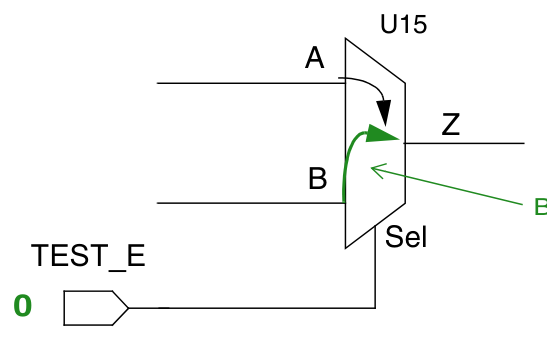
\includegraphics[width=0.9\textwidth]{fig-3-14.png}
  \caption{用常量禁用时序弧}
  \label{fig:3-14}
\end{figure}

\section{禁用时序弧}
\subsection*{Disabling Timing Arcs}

可以用 \cmd{set\_disable\_timing} 禁用路径上的线网或单元时序弧，从而禁用一条时序路径。可以禁用：
\begin{itemize}
  \item 叶级单元或库单元的时序弧。\\
        此时默认禁用到该单元输出的全部时序弧。要禁用单元的某一条时序弧，使用 \opt{-to} 与 \opt{-from}。\\
        例如，下列命令禁用名为 AND3 的库单元到其输出的全部时序弧，以及名为 U17 的单元实例上从引脚 A2 到引脚 ZN 的时序弧：
\begin{lstlisting}
icc2_shell> set_disable_timing my_lib/AND3
icc2_shell> set_disable_timing {U17} -from A2 -to ZN
\end{lstlisting}
  \item 叶级单元引脚、库单元引脚或端口的时序弧。\\
        此时禁用到达以及离开该引脚或端口的全部时序弧。不能用 \opt{-to} 与 \opt{-from} 禁用其中某一条弧。\\
        例如，下列命令禁用名为 U37/A2 与 U51/Z 的叶单元引脚上到达以及离开这些引脚的全部时序弧：
\begin{lstlisting}
icc2_shell> set_disable_timing {U37/A U51/Z}
\end{lstlisting}
\end{itemize}

禁用单元或单元引脚的时序弧时，工具在对应单元上设置 size-only 属性。该属性阻止优化期间删除该单元，但优化期间仍可以调整其尺寸。

要报告 block 中全部被禁用的时序弧，包括由 \cmd{set\_disable\_timing} 禁用的弧，使用 \cmd{report\_disable\_timing}。

\section{使能 preset 与 clear 时序}
\subsection*{Enabling Preset and Clear Timing}

默认情况下，工具不分析这样的时序路径：经过触发器的异步 preset 或 clear 输入，并结束于该触发器的 Q 输出。要在这些路径上使能时序分析与优化，把应用选项 \appopt{time.enable\_preset\_clear\_arcs} 设为 \cmd{true}。
\begin{lstlisting}
icc2_shell> set_app_options -name time.enable_preset_clear_arcs \
    -value true
\end{lstlisting}

\section{data-to-data check 简介}
\subsection*{Introduction to Data-to-Data Checks}

工具可以在设计中任意两个引脚上、在两个都未被定义为时钟的数据信号之间做 setup 与 hold 检查。两个数据（非时钟）信号之间的时序约束称为非时序约束（nonsequential constraint）。该功能可用于检查下列类型的时序约束：
\begin{itemize}
  \item 握手接口逻辑上的约束。
  \item 异步或自定时电路接口上的约束。
  \item 波形异常、难以用 \cmd{create\_clock} 指定的信号上的约束。
  \item 总线各线之间偏斜（skew）的约束。
  \item 异步 preset 与 clear 输入引脚之间的 recovery 与 removal 约束。
\end{itemize}

可以用 \cmd{set\_data\_check} 定义这类检查，也可以在参考库中把它们定义为 nonsequential 约束。只应在前面所述的情形中使用 data check。data check 不应被当作普通时序检查的替代。

下图给出一个带有 nonsequential 约束的单元的简单例子。该单元有两个数据输入 D1 与 D2。D2 的上升沿是有效沿，可能用来锁存 D1 上的数据。引脚 D1 称为被约束引脚（constrained pin），引脚 D2 称为相关引脚（related pin）。

\begin{figure}[htbp]
  \centering
  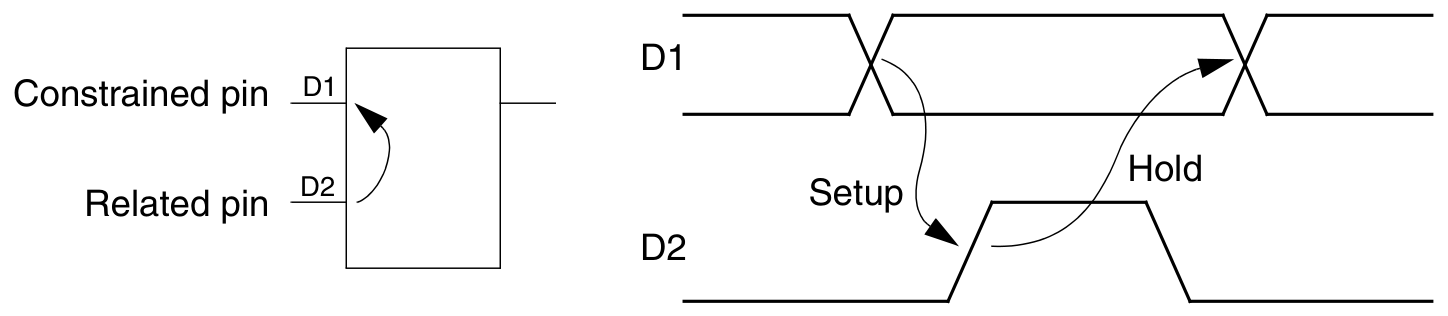
\includegraphics[width=0.9\textwidth]{fig-3-15.png}
  \caption{简单 data check 示例}
  \label{fig:3-15}
\end{figure}

在本例中，D1 上的信号必须在有效沿之前的一段 setup 时间内保持稳定，也必须在有效沿之后的一段 hold 时间内保持稳定。若库单元尚未定义这些 nonsequential 约束，可以用 \cmd{set\_data\_check} 在工具中定义。

data check 是非时序的，因此不会打断时序路径。在下图中，引脚 D1 与 D2 之间的 data check 不会中断虚线箭头所示的时序路径。若把 D2 上的信号定义为时钟，则该检查成为时序检查，路径在 D1 处终止。

\begin{figure}[htbp]
  \centering
  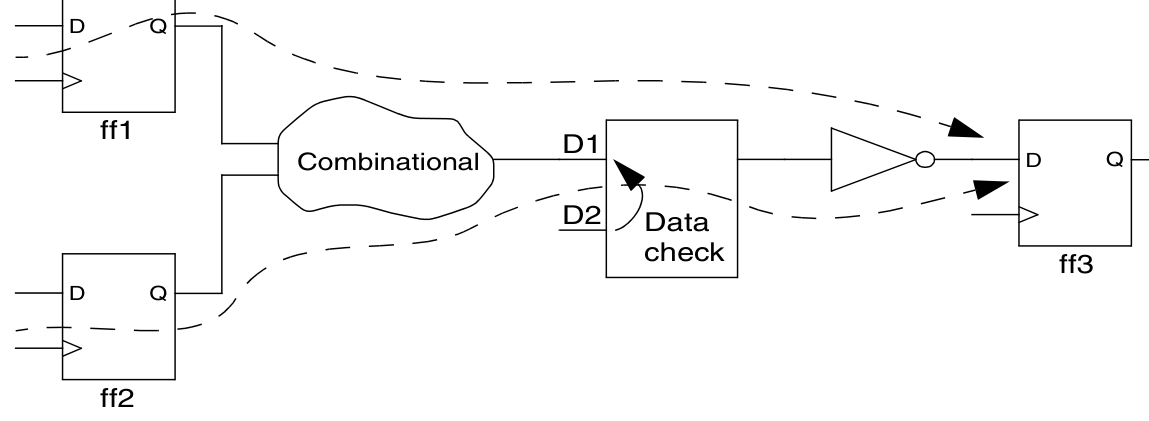
\includegraphics[width=0.9\textwidth]{fig-3-16.png}
  \caption{未被 data check 打断的时序路径}
  \label{fig:3-16}
\end{figure}

在 data check 中，到达被约束引脚或相关引脚的信号可以来自不同时钟域。工具分别检查这些信号路径，并把它们放入不同的时钟组，与普通时序检查相同。

\section{指定 data-to-data check}
\subsection*{Specifying Data-to-Data Checks}

要指定在两个数据引脚之间执行 data-to-data check，按下列方式使用 \cmd{set\_data\_check}：
\begin{itemize}
  \item 用 \opt{-from}、\opt{-rise\_from} 或 \opt{-fall\_from} 把引脚或端口指定为相关引脚。
  \item 用 \opt{-to}、\opt{-rise\_to} 或 \opt{-fall\_to} 把引脚或端口指定为被约束引脚。
  \item 用 \opt{-setup} 或 \opt{-hold} 指定 data check 值只用于 setup 或只用于 hold。否则该值同时用于 setup 与 hold。
  \item 用 \opt{-clock} 指定发射相关引脚上信号的那一个时钟的名称。
\end{itemize}

要去掉用 \cmd{set\_data\_check} 设置的 data check，使用 \cmd{remove\_data\_check}。

\subsection{data check 示例}
\subsubsection*{Examples of Data Checks}

在下图中，D1 上的信号必须在有效沿之前的一段 setup 时间内保持稳定，也必须在有效沿之后的一段 hold 时间内保持稳定。

\begin{figure}[htbp]
  \centering
  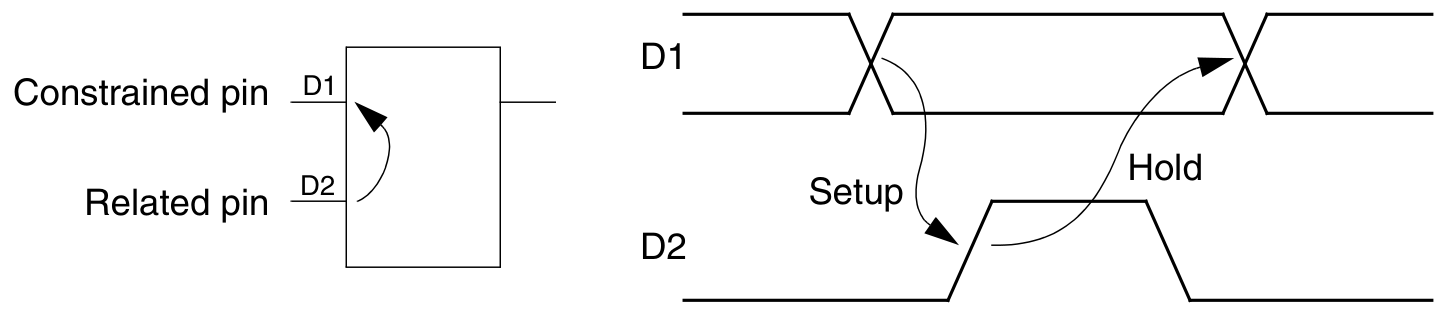
\includegraphics[width=0.9\textwidth]{fig-3-17.png}
  \caption{上升沿上的 data check}
  \label{fig:3-17}
\end{figure}

用下列命令定义这些 data check：
\begin{lstlisting}
icc2_shell> set_data_check -rise_from D2 -to D1 -setup 3.5
icc2_shell> set_data_check -rise_from D2 -to D1 -hold 6.0
\end{lstlisting}

在下图中，data check 同时作用于相关引脚的上升沿与下降沿。

\begin{figure}[htbp]
  \centering
  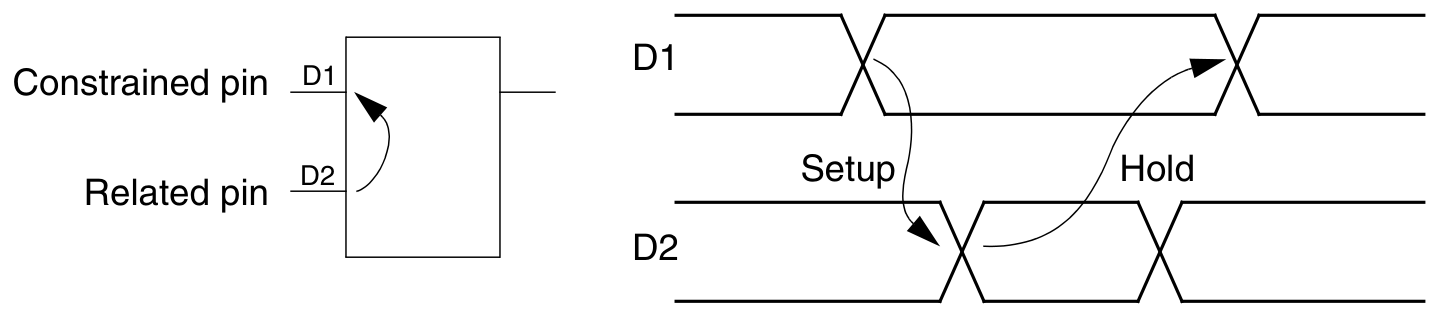
\includegraphics[width=0.9\textwidth]{fig-3-18.png}
  \caption{上升沿与下降沿上的 data check}
  \label{fig:3-18}
\end{figure}

用下列命令定义这些 data check：
\begin{lstlisting}
icc2_shell> set_data_check -from D2 -to D1 -setup 3.5
icc2_shell> set_data_check -from D2 -to D1 -hold 6.0
\end{lstlisting}

可以只指定从上升沿出发的 setup 检查和从下降沿出发的 hold 检查，从而定义 no-change data check，命令如下：
\begin{lstlisting}
icc2_shell> set_data_check -rise_from D2 -to D1 -setup 3.5
icc2_shell> set_data_check -fall_from D2 -to D1 -hold 3.0
\end{lstlisting}

工具把这解释为正脉冲上的 no-change 检查。得到的时序检查如下图所示。

\begin{figure}[htbp]
  \centering
  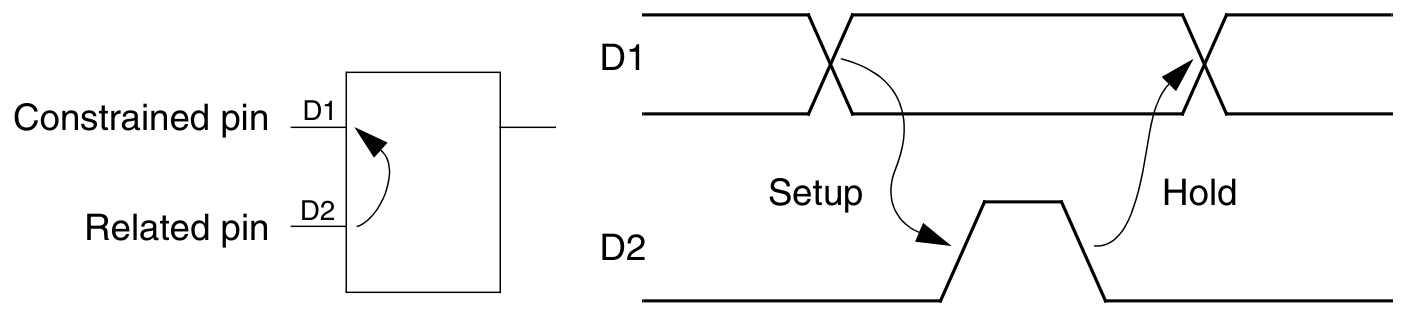
\includegraphics[width=0.9\textwidth]{fig-3-19.png}
  \caption{no-change data check}
  \label{fig:3-19}
\end{figure}

\section{使能基于库的 data check}
\subsection*{Enabling Library-Based Data Checks}

若相关引脚上的信号未被定义为时钟，要让工具对库单元中定义了 nonsequential 时序约束的任何单元执行 data check，把应用选项 \appopt{time.enable\_non\_sequential\_checks} 设为 \cmd{true}，如下例所示：
\begin{lstlisting}
icc2_shell> set_app_options -name time.enable_non_sequential_checks \
    -value true
\end{lstlisting}

该变量默认为 \cmd{false}。

\begin{noteBox}
这一行为与 PrimeTime 不同。PrimeTime 始终执行 nonsequential arc 检查。
\end{noteBox}

若相关引脚上的信号被定义为时钟，工具忽略库中定义的 nonsequential 时序约束。

在单元库中，单元的 nonsequential 约束通过指定相关引脚，并为被约束引脚赋予下列 \cmd{timing\_type} 属性来定义：
\begin{itemize}
  \item \cmd{non\_seq\_setup\_rising}
  \item \cmd{non\_seq\_setup\_falling}
  \item \cmd{non\_seq\_hold\_rising}
  \item \cmd{non\_seq\_hold\_falling}
\end{itemize}

\begin{seeAlsoBox}
关于在库中定义 nonsequential 约束的更多信息，参见 Library Compiler 文档。
\end{seeAlsoBox}

使用库单元中定义的 nonsequential 约束，比使用 \cmd{set\_data\_check} 得到的分析更准确，因为 setup 与 hold 时间可以随被约束引脚和相关引脚的 slew 变化。\cmd{set\_data\_check} 对 slew 不敏感。

\cmd{remove\_data\_check} 不会去掉库单元中定义的 data check。

\section{时钟门控检查简介}
\subsection*{Introduction to Clock-Gating Checks}

当时钟网络中含有反相器或缓冲器以外的逻辑时，就出现门控时钟信号。工具不会自动检查时钟门控单元的门控信号上的 setup 与 hold 违例。因此，这些信号有可能在时钟脉冲穿过门控单元时发生跳变，从而既产生被削窄的时钟脉冲，也产生虚假的时钟脉冲。

下图给出：在没有时钟门控检查时，时钟门控输入上的非法变化可能造成的畸变时钟波形。

\begin{figure}[htbp]
  \centering
  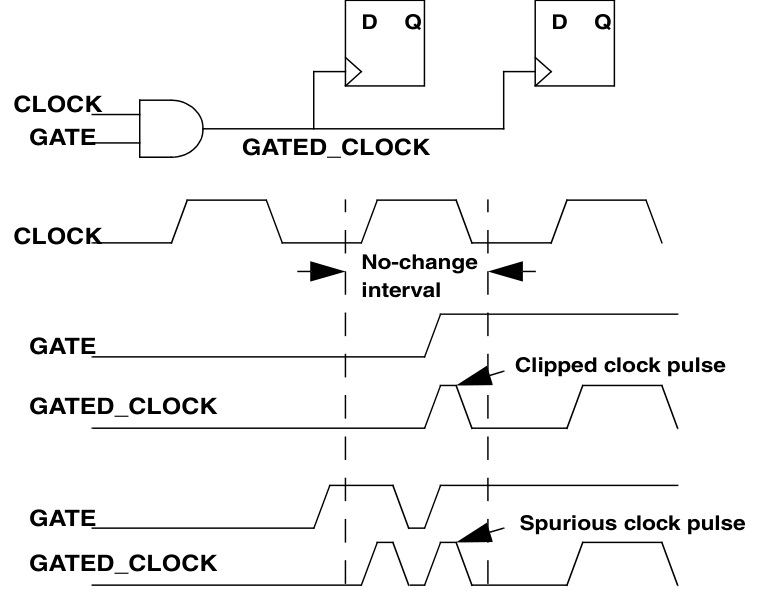
\includegraphics[width=0.9\textwidth]{fig-3-20.png}
  \caption{畸变的时钟波形}
  \label{fig:3-20}
\end{figure}

要控制门控信号的跳变，可以用 \cmd{set\_clock\_gating\_check} 相对于时钟指定 setup 裕量与 hold 裕量。

下图给出在作为门控元件的 AND 或 NAND 门上执行的时钟门控检查。

\begin{figure}[htbp]
  \centering
  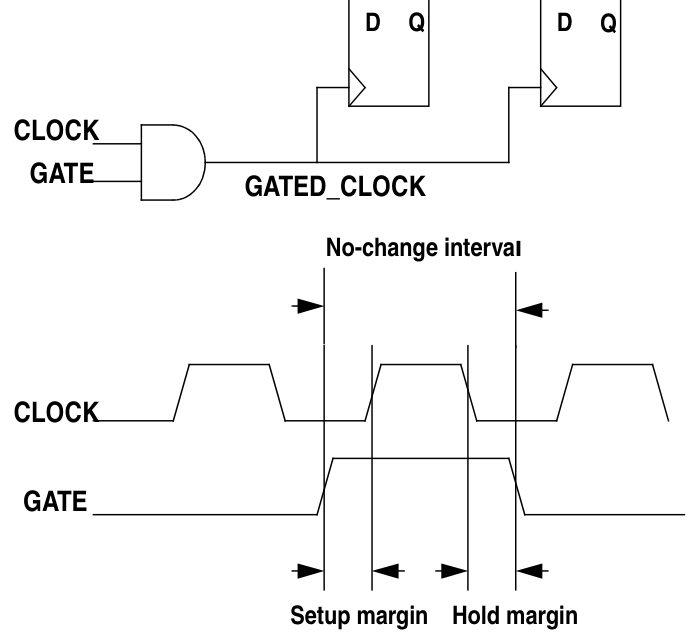
\includegraphics[width=0.9\textwidth]{fig-3-21.png}
  \caption{AND 与 NAND 门的时钟门控检查}
  \label{fig:3-21}
\end{figure}

下图给出在作为门控元件的 OR 或 NOR 门上执行的时钟门控检查。

\begin{figure}[htbp]
  \centering
  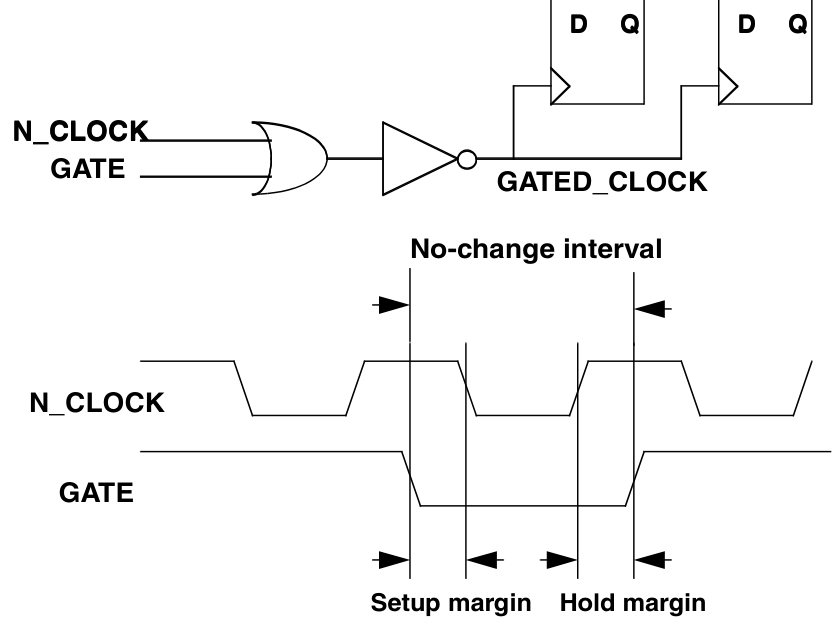
\includegraphics[width=0.9\textwidth]{fig-3-22.png}
  \caption{OR 与 NOR 门的时钟门控检查}
  \label{fig:3-22}
\end{figure}

\section{指定时钟门控检查}
\subsection*{Specifying Clock-Gating Checks}

要指定时钟门控检查，使用 \cmd{set\_clock\_gating\_check}。

使用该命令时，工具默认：
\begin{itemize}
  \item 对当前 block 的全部时钟门控元件执行时钟门控检查。\\
        要把检查限制到指定单元、指定时钟，或某个端口或引脚的传递扇出（transitive fanout），指定所需对象。
  \item 使用的 setup 与 hold 值为零。要设置具体的 setup 或 hold 值，使用 \opt{-setup} 或 \opt{-hold}。
  \item 同时约束门控信号的上升沿与下降沿。\\
        若只控制上升沿或下降沿，使用 \opt{-rise} 或 \opt{-fall}。
  \item 根据门控逻辑，决定用时钟的高电平还是低电平来约束门控信号。\\
        若门控单元是：
        \begin{itemize}
          \item AND 或 NAND 门，工具在时钟的高电平上执行检查。
          \item OR 或 NOR 门，工具在时钟的低电平上执行检查。
          \item 其他门，除非指定使用时钟的哪一个电平，否则工具不执行检查。
        \end{itemize}
        要指定在时钟的哪一个电平上执行检查，使用 \opt{-high} 或 \opt{-low}。
\end{itemize}

工具像处理其他时序约束一样处理时钟门控检查，并尝试调整驱动门控输入的逻辑延迟，以避免 setup 与 hold 违例。优化期间，对带有时钟门控检查的单元，工具只能调整尺寸。

时钟门控检查只能在一个时钟信号与一个非时钟信号之间进行，不能在两个时钟信号之间进行，也不能在两个非时钟信号之间进行。

要去掉时钟门控检查，使用 \cmd{remove\_clock\_gating\_check}。

可以用 \cmd{set\_disable\_clock\_gating\_check} 列出希望工具忽略的单元和引脚，从而在指定单元和引脚上禁用时钟门控检查。要取消该命令的作用，使用 \cmd{remove\_disable\_clock\_gating\_check}。

下例说明如何在 CLK1 时钟网络中的全部门上指定 setup 要求 0.2 与 hold 要求 0.4。
\begin{lstlisting}
icc2_shell> set_clock_gating_check -setup 0.2 -hold 0.4 CLK1
\end{lstlisting}
